% !TEX TS-program = xelatex
% !BIB TS-program = bibtex
\documentclass[12pt,letterpaper]{article}
\usepackage{style/dsc180reportstyle} % import dsc180reportstyle.sty
\usepackage{listings}

\lstdefinestyle{python}{
    language=Python,
    basicstyle=\ttfamily\footnotesize,
    showstringspaces=false,
    breaklines=true
}

%%%%%%%%%%%%%%%%%%%%%%%%%%%%%%%%%%%%%%%%%%%%%%%%%%%%%%%%
%%%% Title and Authors
%%%%%%%%%%%%%%%%%%%%%%%%%%%%%%%%%%%%%%%%%%%%%%%%%%%%%%%%

\title{Predicting Financial Transaction Categories: A Comparative Analysis of Machine Learning Based Methods for Optimal Classification}

\author{
\begin{tabular}[t]{ccc}
Brandon Dioneda & Mert Ozer & Qianjin Zhou \\
{\tt bdioneda@ucsd.edu} & {\tt mozer@ucsd.edu} & {\tt q9zhou@ucsd.edu}
\end{tabular}
\\[4ex]
\begin{tabular}[t]{ccc}
Brian Duke (Mentor) & Kyle Nero (Mentor) & Berk Ustun (Mentor)\\
{\tt brian.duke@prismdata.com} & {\tt kyle.nero@prismdata.com} & {\tt berk@ucsd.edu}
\end{tabular}
}

\begin{document}
\maketitle

%%%%%%%%%%%%%%%%%%%%%%%%%%%%%%%%%%%%%%%%%%%%%%%%%%%%%%%%
%%%% Abstract and Links
%%%%%%%%%%%%%%%%%%%%%%%%%%%%%%%%%%%%%%%%%%%%%%%%%%%%%%%%


\begin{abstract}
    \textcolor{LightGrey}{Evaluating creditworthiness has been a challenge since the 19th century, with FICO scores becoming the most widely used metric today. However, traditional credit scoring models often overlook consumers who lack conventional credit history, leading to unequal access to credit. With the advent of digital technology, alternative data sources now offer the opportunity for more inclusive credit assessments. This project addresses these gaps by analyzing non-personal financial information, such as categorizing bank transactions and predicting personal income to assess creditworthiness more fairly.}
\end{abstract}

\begin{center}
Code: \url{https://github.com/mozer123/credit_score/}
\end{center}

\maketoc
\clearpage

%%%%%%%%%%%%%%%%%%%%%%%%%%%%%%%%%%%%%%%%%%%%%%%%%%%%%%%%
%%%% Main Contents
%%%%%%%%%%%%%%%%%%%%%%%%%%%%%%%%%%%%%%%%%%%%%%%%%%%%%%%%

\section{Introduction}
\subsection{Background Information}
    {Creditworthiness assessment has been a longstanding challenge, and while modern credit scores became widely adopted in 1989, these traditional models often fail to account for the financial profiles of individuals who lack conventional credit histories. As a result, millions are excluded from fair access to credit. Moreover, early credit evaluations were frequently marred by discriminatory practices, factoring in age, race, and marital status, while even today, reliance on conventional credit history can reinforce socioeconomic biases. 

    This project leverages bank data from 2017-2023 to develop a fairer, non-discriminatory model for assessing credit risk. By categorizing individual bank transactions and predicting personal income as alternative indicators, our approach emphasizes unbiased and responsible credit assessments, aiming to expand equal access to credit.
    }
\subsection{Literature Review and Discussion of Prior Work}
    {In their review, \cite{markov2022credit} discuss the evolving trends in credit scoring methodologies, highlighting the shift from traditional statistical methods, such as logistic regression, toward more complex machine learning models, including decision trees, neural networks, and ensemble methods. The authors emphasize the growing popularity of explainable AI (XAI) in credit scoring, as financial institutions are required to provide transparency in their decision-making processes, especially in highly regulated environments. They also underscore the importance of considering biases in model training, especially when alternative data sources are involved, as biased data can lead to discriminatory credit outcomes. This work sets the stage for understanding the inherent challenges in balancing model accuracy and fairness, particularly when advanced techniques are employed.
        
    \cite{litty2024beyond} explores the integration of alternative data sources, such as social media behavior, mobile phone usage patterns, and even psychometric data, in credit risk assessment models. These sources offer the potential to improve credit scoring accuracy, especially for individuals with limited or no traditional credit history, thus addressing the issue of financial inclusion. Litty’s work outlines the effectiveness of AI-powered models in capturing complex relationships within these unstructured data sources, which are often ignored in conventional credit scoring models. Furthermore, Litty’s research identifies the potential risks of privacy invasion and data security when using personal and behavioral data, suggesting that such risks must be carefully managed to avoid ethical concerns.
    
    Together, these studies highlight the transformative role of AI in credit scoring, offering insights into both the benefits and challenges of these new methods. Unlike traditional models that rely on static financial data, our approach leverages natural language processing (NLP) on transaction memos and additional data sources to develop a more holistic view of consumer behavior. By focusing on these unstructured transaction details, we aim to extract latent features that may reveal patterns of financial responsibility not captured in traditional scoring systems. This approach not only improves the granularity of credit assessment but also offers a pathway to more personalized credit models, contributing to ongoing efforts in making credit scoring more inclusive and responsive to diverse financial behaviors.
    }
    
\subsection{Description of Relevant Data}
{Consumers' bank transactions provided by PrismData which are from years 2017-2023:}
\begin{itemize}
    \item {Inflows.pqt: Contains transaction-level information on inflowing transactions (such as: paychecks, refunds, etc.)}
    \begin{figure}[H]
        \centering
        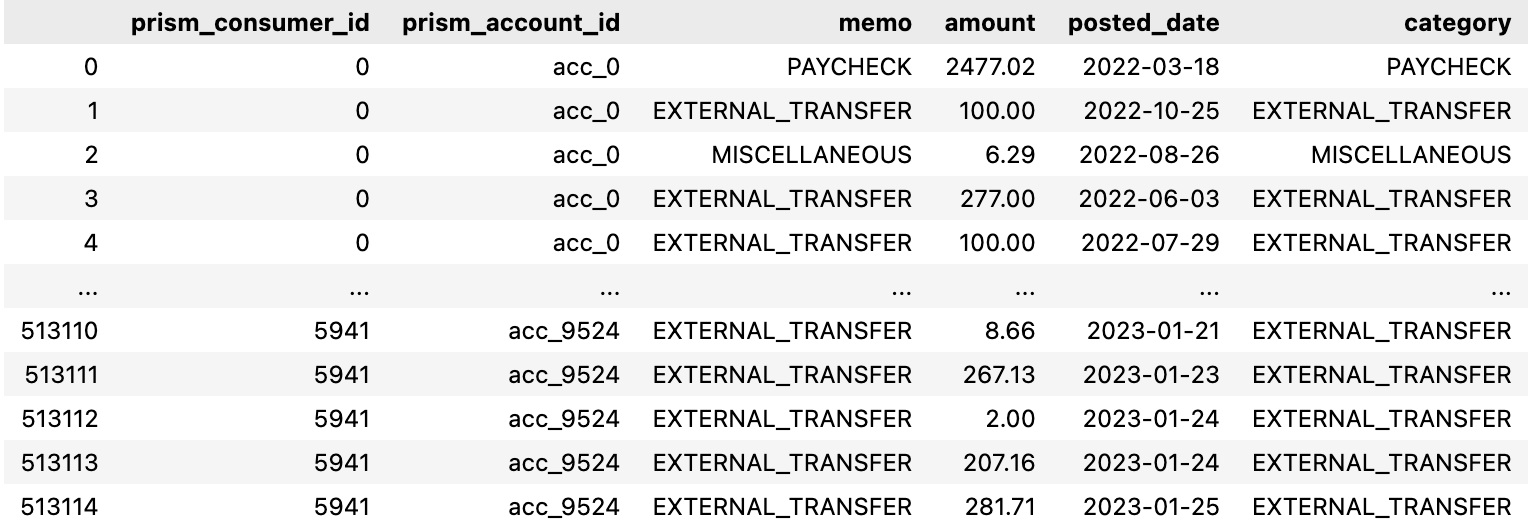
\includegraphics[width=0.6\textwidth]{figure/inflows.png}
        \caption{Inflows.pqt}
        \label{fig:enter-label}
    \end{figure}
    
    \item {Outflows.pqt: Contains transaction-level information on outflowing transactions (such as: groceries, rent, etc.)}
    \begin{figure}[H]
        \centering
        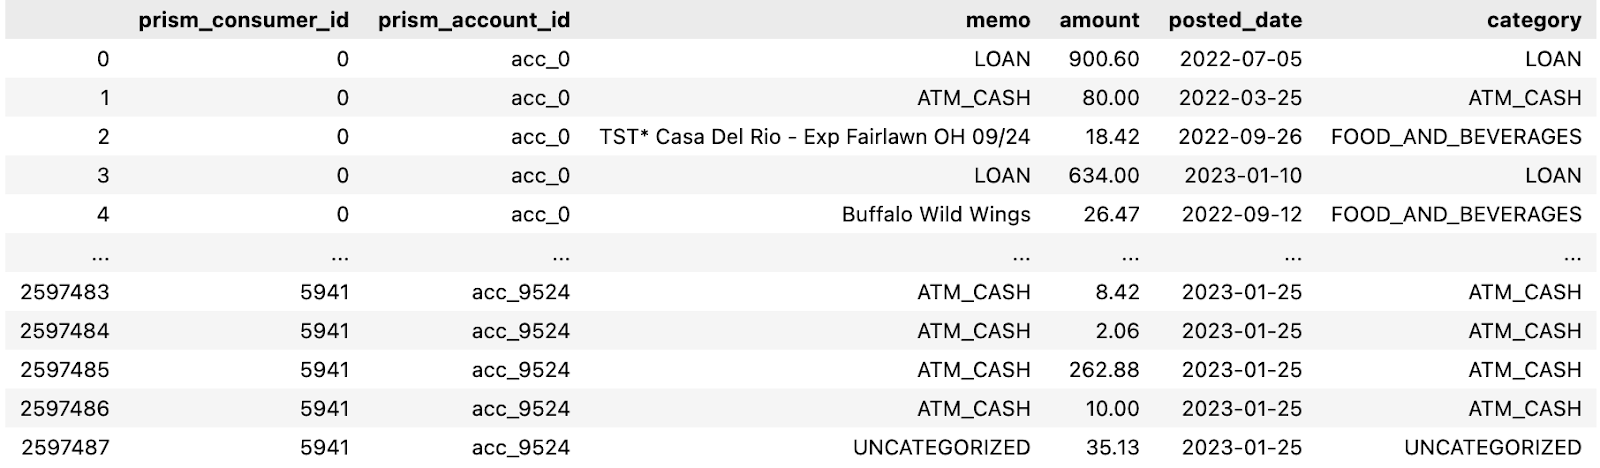
\includegraphics[width=0.6\textwidth]{figure/outflows.png}
        \caption{Outflows.pqt}
        \label{fig:enter-label}
    \end{figure}
    
\end{itemize}
Columns:
\begin{itemize}
    \item {prism\_consumer\_id: ID associated with the consumer}
    \item {prism\_account\_id: ID associated with the account}
    \item {memo: Descriptive text for the transaction}
    \item {amount: Transaction amount}
    \item {posted\_date: Date when the transaction was posted}
    \item {category: Type/category of the transaction}
\end{itemize}

\section{Methods}
\subsection{Exploratory Data Analysis and Bias Checking}
\begin{enumerate}
    \item{\textbf{Summary Statistics of Transaction Amounts:}
    
    The variable (transaction) "amount” is important information that could potentially help us build our models, hence we calculated the summary statistics of “amount” for both inflow and outflow datasets.}
    \begin{itemize}
        \item {Inflow Data:}
            \begin{itemize}
                \item{Count: 513,115 transactions}
                \item{Mean amount: \$734.70}
                \item{Median amount: \$100.00}
                \item{Standard deviation: \$5,296.57}
                \item{Range: \$0.01 to \$1,154,966.00}
            \end{itemize}
    
        \item {Outflow Data:}
            \begin{itemize}
                \item{Count: 2,597,488 transactions}
                \item{Mean amount: \$145.13}
                \item{Median amount: \$24.26}
                \item{Standard deviation: \$1,697.88}
                \item{Range: \$0.00 to \$654,853.20}
            \end{itemize}
    \end{itemize}
{As shown in the summary statistics above,  inflows tend to have higher transaction amounts compared to outflows, with a significant difference in mean and maximum values.}

    \item{\textbf{Category Distribution:}}
    \begin{figure}[H]
        \centering
        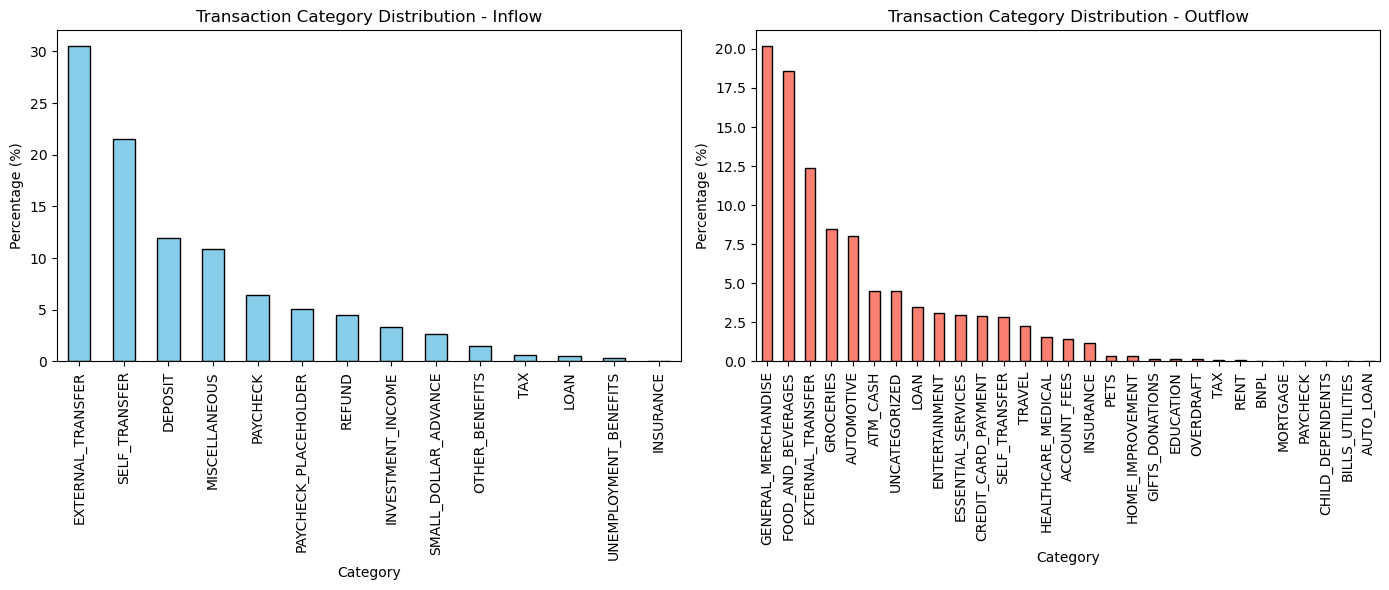
\includegraphics[width=1.0\textwidth]{figure/category_dist.png}
        \caption{Category Distribution}
        \label{fig:enter-label}
    \end{figure}
    \begin{itemize}
        \item Inflow Data: Most common categories are EXTERNAL\_TRANSFER $(30.5\%)$ and SELF\_TRANSFER $(21.5\%)$.
        \item Outflow Data: Most common categories are GENERAL\_MERCHANDISE $(20.2\%)$, FOOD\_AND\_BEVERAGES $(18.6\%)$, and EXTERNAL\_TRANSFER $(12.4\%)$.
    \end{itemize}

    {We also computed the most common merchants(“memo”) per category for the outflow dataset. The results for the inflow dataset are not displayed because all memos exactly match their categories.}
    \begin{figure}[H]
        \centering
        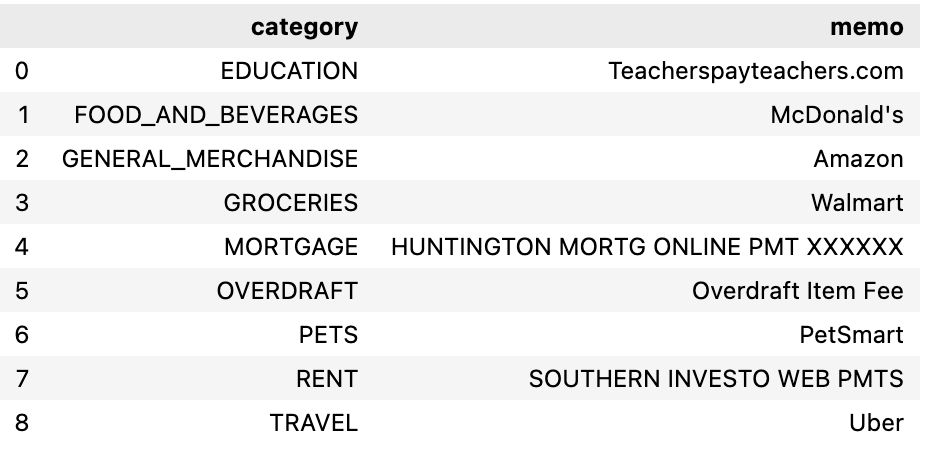
\includegraphics[width=0.4\textwidth]{figure/cmn_merchant.png}
        \caption{Most Common Merchant per Category - Outflow Dataset}
        \label{fig:enter-label}
    \end{figure}
    {We can see that McDonald’s, Amazon, Walmart, Uber, etc. are the most common merchants for each category they belong to (see Figure 4). It is worth noting that the process of finding the most common merchant is based on the uncleaned “memo” column.}
\end{enumerate}

\subsection{Data Cleaning}
{To prepare our dataset for further analysis and modeling, we cleaned the memo column.}
{Here is how we cleaned the memo with considerations we made along the way:}

\begin{itemize}
    \item Filtered rows where the memo field differs from the category field, which would allow our future models to look for more meaningful features 
    \item The resulting unique categories are: ['FOOD\_AND\_BEVERAGES', 'GENERAL\_MERCHANDISE', 'GROCERIES', 'PETS', 'TRAVEL', 'MORTGAGE', 'OVERDRAFT', 'EDUCATION', 'RENT']
    \item Converted all bank memos to lowercase
    \item Removed special characters and numbers to focus on text-based features
    \item Removed placeholders (e.g., sequences like "xxx")
    \item Trimmed extra spaces to clean up the text field further
\end{itemize}
\begin{figure}[H]
    \centering
    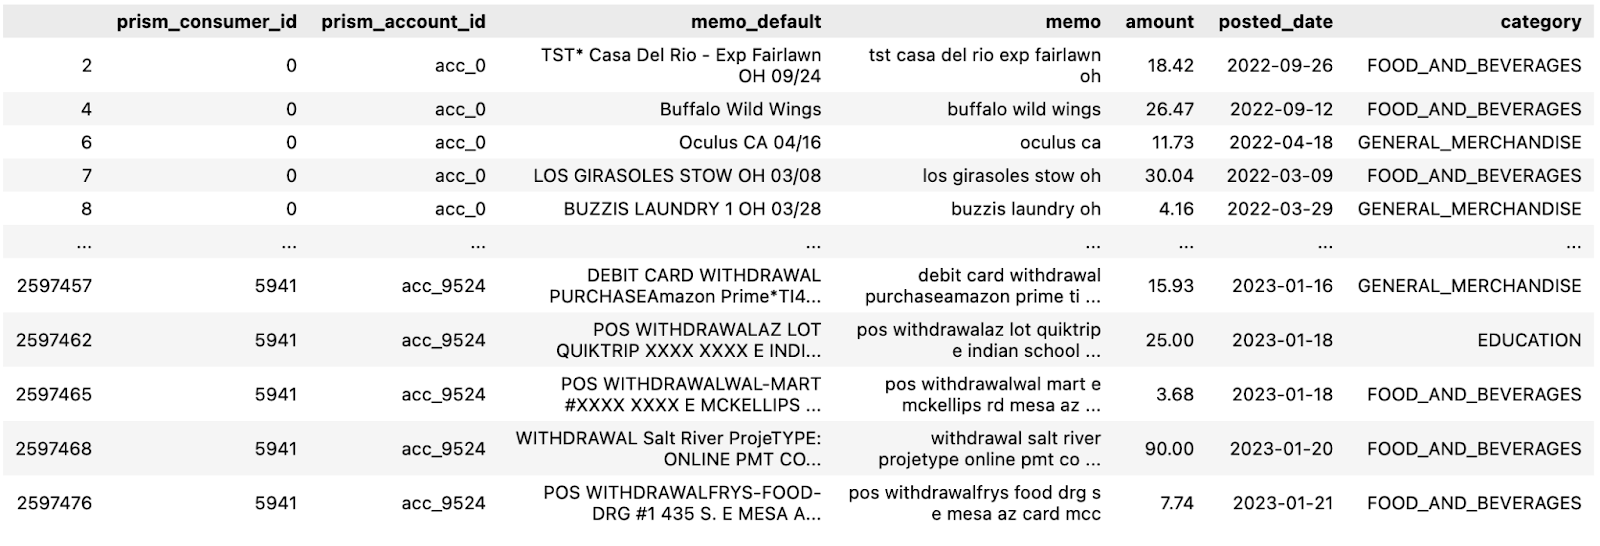
\includegraphics[width=1.0\textwidth]{figure/memo_clean.png}
    \caption{Original Memos vs Cleaned Memos}
    \label{fig:enter-label}
\end{figure}

\subsection{Feature Engineering}
\begin{itemize}
    \item {Features based on Memo:}
        \begin{itemize}
            \item {TF-IDF}: Process that helps pick out the most distinctive and meaningful words from the bank memos. Some words are present in certain transaction types. For example, the term "nsf" (which stands for "non-sufficient funds") is only present in OVERDRAFT transactions
        \end{itemize}
    \item {Features based on Date:}
        \begin{itemize}
            \item 
                \texttt{date\_month}: Indicates the month that a transaction was processed.            
            \item 
                \texttt{date\_day}: Indicates the weekday that a transaction was processed. 
                
            \item 
                \texttt{date\_weekend}: Indicates if a transaction was processed on a weekend. Certain transactions are never processed over Saturday/Sunday.
        \end{itemize}
    \item {Features based on Amount:}
        \begin{itemize}
            \item 
                \texttt{is\_whole\_num:}: Indicates whether a transaction amount is a whole number. This can provide insight into the nature of the transaction—for example, most food and beverage transactions typically have fractional amounts, whereas rent payments are often whole numbers. 
        \end{itemize}
\end{itemize}

\subsection{Models for Categorization}
These are the various methods we tried using as a way to categorize an individual's bank transactions. We believe that being able to accurately categorize one’s bank transactions helps us gain insight into people’s financial behavior. How do they spend their money? What do they spend it on? By answering these questions, we aim to build a clearer picture of an individual’s financial stability and habits, ultimately enabling a more reliable assessment of their creditworthiness.
\paragraph{Traditional Classifiers:}
    \begin{enumerate}
        \item {Logistic Regression as a Baseline}
            \begin{itemize}
                \item {Logistic Regression was used as a starting point for comparison, since it is easily to implement and prediction time is relatively fast}
                \item {Simply used default parameters from sklearn Logistic Regression that only used TF-IDF on the memo column for features}
            \end{itemize}
        \item {FastText}
            \begin{itemize}
                \item {FastText is a lightweight and efficient text classification library by Facebook. It treats text data as a bag of words or bag of n-grams, providing a simple but effective approach for capturing word relationships and context}
                \item {We processed the data to align with the format required by the FastText model and trained the model with hyperparameters (epoch=30, lr=0.1, wordNgrams=2) optimized through grid-search and cross-validation}
            \end{itemize}
        \item {XGBoost}
            \begin{itemize}
                \item{We also attempted our predictive task with the gradient-boosted decision tree model from the \textit{xgboost} library. XGBoost excels in structured data tasks. It captures complex feature interactions and is optimized for speed and accuracy. The XGBoost classifier was trained using TF-IDF features derived from the memo text data.}
            \end{itemize}
    \end{enumerate}

\paragraph{Large Language Models (LLMs):}

\begin{enumerate}
        \item {DistilBERT}
            \begin{itemize}
                \item {DistilBERT is a lightweight transformer model derived from BERT, designed to retain most of BERT’s accuracy while being faster and more efficient. It utilizes deep contextual embeddings to understand semantic relationships in text, making it effective for text classification tasks.}
                \item {The dataset was reduced to 12,500 rows due to computational resource constraints (see Table 1). DistilBERT was fine-tuned for the task using the Hugging Face library, with hyperparameters including 3 epochs of training. The model leveraged pre-trained weights and adapted them to the transaction classification task.}
            \end{itemize}
        \item {Few Shot Learning}
            \begin{itemize}
                \item {We utilized the open-source model Nemotron 70B from NVIDIA. Each prompt included five examples demonstrating the desired response format and predefined category options. Inference was conducted via an API service rather than being hosted locally.}
            \end{itemize}
        \item {Fine-Tuning}
            \begin{itemize}
                \item{We employed an instruct version of the open-source model Llama-3.2-1B from Meta for this task. To optimize the fine-tuning process, we leveraged Unsloth, a library designed to enhance processing speed and reduce memory consumption. The fine-tuning was conducted in the Google Colab environment.}
            \end{itemize}
    \end{enumerate}


\vspace{10cm} 

\subsection{Income}
{We analyzed the inflows dataset further to investigate consumer’s income. Doing this would help us answer questions like: Does this person have a steady inflow of money to be able to pay their bills? Do they have an income in the first place? \\ \\ Major sources of income that we want to utilize later:}
\begin{itemize}
    \item {DEPOSIT}: 20.2\%
    \item {EXTERNAL\_TRANSFERS}: 51.5\%
    \item {INVESTMENT\_INCOME}: 5.7\%
    \item {OTHER\_BENEFITS}: 2.5\%
    \item {PAYCHECK}: 19.5\%
    \item {UNEMPLOYMENT\_BENEFITS}: 0.6\%
\end{itemize}

\begin{figure}[H]
    \centering
    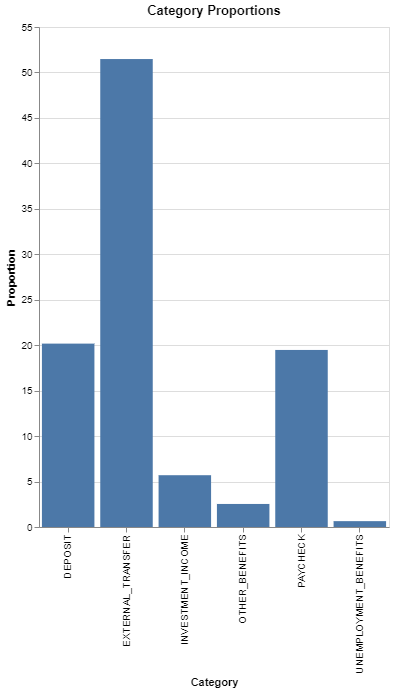
\includegraphics[width=0.5\textwidth]{figure/income.png}
    \caption{Income Categories Distribution}
    \label{fig:enter-label}
\end{figure}



\section{Results}

\vspace{0.5cm} 

\begin{table}[H]
    \centering
    \begin{tabular}{|l|p{2.5cm}|p{1.7cm}|p{3.5cm}|p{2.5cm}|p{1.7cm}|}
    \hline
    \textbf{Model}           & \textbf{Training Dataset Size} & \textbf{Training Time (s)} & \textbf{Inference (predictions per second)} & \textbf{Testing Dataset Size} & \textbf{Accuracy (\%)} \\ \hline
    Logistic Regression      & 979,839                        & 32.8                       & 326,613                                     & 326,613                      & 96.45                 \\ \hline
    FastText                 & 969,666                        & 19.1              & 336,786                            & 336,786                     & 96.88        \\ \hline
    XGBoost                  & 969,666                        & 30.9                       & 300,000                                     & 336,786                      & 91.98                 \\ \hline
    DistilBERT               & 12,500                         & 600                        & 54.67                                       & 12,500                       & 89.56                 \\ \hline
    Nemotron 70B             & 5                              & N/A                        & 0.44                                        & 100                          & 78.00                 \\ \hline
    Llama-3.2-1 B            & 1,000                          & 72                         & 3.04                                        & 100                          & 75.00                 \\ \hline
    \end{tabular}
    \caption{Performance comparison of models on transaction categorization.}
    \label{tab:model_comparison}
\end{table}


\section{Discussion}
\subsection{Traditional Classifiers}

The performance comparison between Logistic Regression, FastText, and XGBoost reveals interesting trade-offs among accuracy, training time, and inference speed. As seen in Table 1, FastText achieved the highest accuracy at 96.88\%, outperforming both Logistic Regression (96.45\%) and XGBoost (91.98\%).

FastText had the fastest training time at 19.1 seconds, making it highly efficient for large-scale datasets like this one. Its inference speed was also the fastest, processing approximately 336,786 predictions per second.

XGBoost lagged behind in accuracy at 91.98\% and had a slower inference speed of 300,000 predictions per second, despite a reasonable training time of 30.9 seconds.

Overall, FastText stands out as the best-performing model in terms of accuracy, speed, and scalability, making it an excellent choice for text-based transaction classification tasks.


\subsection{Thoughts on LLMs}

Ideally, we aim for a local solution that offers high accuracy and fast inference while minimizing computational resource requirements. Although longer training times can be a drawback during testing different parameters, this is more acceptable compared to other factors, as the model will only need to be trained once in the production phase.

 While inference speeds we have may reflect that LLM solutions are not useful to work with real data in a timely manner, hosting the model locally on a supercomputer can significantly improve processing capabilities. However, accuracy remains a concern, as the LLM with few-shot learning often generates generic responses based on its pre-trained knowledge. For instance, we observed it predicting "GENERAL\_MERCHANDISE" more frequently than appropriate.
 
Fine-tuning the LLMs could address the accuracy issues associated with few-shot learning. However, achieving higher accuracy has been difficult due to the substantial computational resources required for fine-tuning. Despite this, the approach demonstrates promise: even when we utilized a much smaller model, it performed comparably to a larger model without fine-tuning.


\section{Conclusion}
Our study highlights FastText as the most effective model for categorizing financial transactions, achieving superior accuracy (96.88\%), efficient training, and rapid inference compared to Logistic Regression and XGBoost. While Logistic Regression provided a reliable baseline, XGBoost, despite its utility in structured data tasks, underperformed in this context. Large Language Models (LLMs) demonstrated potential, but their practical application was limited by high computational costs and slower inference speeds.  

Compared to prior works, our results align with \cite{markov2022credit}, who noted the growing efficiency of advanced machine learning models over traditional approaches like Logistic Regression in financial applications. However, unlike their findings on decision tree-based models, XGBoost underperformed in our task, likely due to its inability to fully leverage the unstructured text features in transaction memos. Similarly, while \cite{litty2024beyond} emphasized the transformative role of AI-powered models incorporating alternative data sources, our work demonstrates that simpler models like FastText can outperform resource-intensive methods such as LLMs. Additionally, our focus on categorizing financial transactions based on bank memos complements Litty’s findings by providing a practical and interpretable method for assessing financial behavior.  

However, our approach is not without limitations. Our reliance on pre-defined transaction categories may miss subtle patterns in unstructured financial data. Furthermore, the computational constraints prevented extensive exploration of LLM fine-tuning, which may have improved their accuracy and generalizability. Finally, while FastText offers excellent scalability, its simplistic representations may not capture nuanced semantic relationships as effectively as LLMs.  

Future work should focus on integrating alternative features, such as behavioral patterns or temporal trends, to enhance model performance. For instance, expanding the analysis of the income section could provide valuable insights. By measuring the regularity of inflows—such as the consistency, frequency, and source of transactions—we can better determine whether a particular transaction qualifies as actual income. This refinement could improve the reliability of creditworthiness assessments by distinguishing between steady income streams and irregular inflows.

 Researchers building on our work could explore hybrid models that merge FastText's speed and interpretability with the contextual depth of LLMs, effectively bridging the gap between efficiency and complexity for more robust transaction classification. Incorporating income regularity analysis into these hybrid models could further enhance their predictive capabilities, offering deeper and more nuanced financial insights.
%%%%%%%%%%%%%%%%%%%%%%%%%%%%%%%%%%%%%%%%%%%%%%%%%%%%%%%%
%%%% Reference / Bibliography
%%%%%%%%%%%%%%%%%%%%%%%%%%%%%%%%%%%%%%%%%%%%%%%%%%%%%%%%
\bibliography{reference}
\bibliographystyle{style/dsc180bibstyle}
\end{document}